\documentclass[10pt]{article}
\usepackage{titlesec}
\usepackage{geometry}
\geometry{verbose,tmargin=.9in,bmargin=.9in,lmargin=1.0in,rmargin=1.0in}
\usepackage{amsmath,amsfonts,amsthm,amssymb}
\usepackage{url}
\usepackage{color}
\usepackage[usenames,dvipsnames,svgnames,table]{xcolor}
\usepackage[colorlinks=true, linkcolor=red, urlcolor=blue, citecolor=gray]{hyperref}
\usepackage{float}
\usepackage{caption}
\usepackage{subcaption}
\usepackage{graphicx}
\usepackage{wrapfig}
\usepackage{booktabs}
\usepackage{longtable}
\usepackage{enumitem}
\usepackage{multicol}
\usepackage{etoolbox}

\definecolor{nyuDarkPurple}{HTML}{330662}
\definecolor{nyuOfficialPurple}{HTML}{57068c}

\newcommand{\spara}[1]{\vspace{.5em}\noindent {\large\sffamily\textcolor{nyuOfficialPurple}{#1}}}
\titleformat{\section}[hang]{\Large\sffamily\color{nyuDarkPurple}}{\thesection}{1em}{}
\titleformat{\subsection}[hang]{\large\sffamily\color{nyuDarkPurple}}{\thesection}{1em}{}
\titleformat{\subsubsection}[hang]{\normalsize\sffamily\color{gray}}{\thesection}{1em}{}

\usepackage{fancyhdr}
\pagestyle{fancy}
\lhead{
\includegraphics[width=4cm]{tandon_long_color.eps}}
\rhead{\thepage}
\pagenumbering{gobble}

\setcounter{secnumdepth}{0}

% math commands
\DeclareMathOperator{\R}{\mathbb{R}}
\newcommand{\E}{\mathbb{E}}
\DeclareMathOperator{\Var}{Var}
\newcommand{\bs}[1]{\boldsymbol{#1}}
\newcommand{\bv}[1]{\mathbf{#1}}

\usepackage{bbm}

\begin{document}
	
\begin{center}
	\normalsize
	New York University Tandon School of Engineering
	
	Computer Science and Engineering
	\medskip
	
	\large
	CS-GY 6763: Homework 2. 
	
	Due Tuesday, October 18th, 2022, 11:59pm ET.
	\medskip
	
	\normalsize 
	\noindent \emph{Collaboration is allowed on this problem set, but solutions must be written-up individually. Please list collaborators for each problem separately, or write ``No Collaborators" if you worked alone.}

\end{center} 

\subsection{Problem 1: Analyzing Sign-JL and JL for Inner Products }
\textbf{(20 pts)}
Often practitioners prefer JL matrices with discrete random entries instead of Gaussians because they take less space to store and are easier to generate. We  analyze one construction below.

Suppose that $\bs{\Pi}$ is a ``sign Johnson-Lindenstrauss matrix'' with $n$ columns, $k$ rows, and i.i.d. $\pm 1$ entries scaled by $1/\sqrt{k}$. In other words, each entry in the matrix has values $-1/\sqrt{k}$ with probability $1/2$ and $1/\sqrt{k}$ with probability $1/2$.
\begin{enumerate}
	\item Prove that for any vector $\bv{x}\in \R^n$, $\E[\|\bs{\Pi}\bv{x}\|_2^2] = \|\bv{x}\|_2^2$ and that $\Var[\|\bs{\Pi}\bv{x}\|_2^2] \leq \frac{2}{k}\|\bv{x}\|_2^4$. This is the meat of the problem and will take some effort. 
	\vspace{.5em}

	
	\item Use the above to prove that $\Pr\left[\left|\|\bs{\Pi}\bv{x}\|_2^2 - \|\bv{x}\|_2^2\right| \geq \epsilon\|\bv{x}\|_2^2 \right] \leq \delta$ as long as we choose $k = O\left(\frac{1/\delta}{\epsilon^2}\right)$. Note that this bound almost matches the distributed JL lemma proven in class, but with a worse failure probability dependence of $1/\delta$ in place of $\log(1/\delta)$. 
	\vspace{.5em}
	
	\textit{With more work, it's possible to improve the dependence to $\log(1/\delta)$ for the sign-JL matrix, but we won't do so here.}
	
	\item Generalize your analysis above to show that JL matrices are also useful in approximating inner products between two vectors. For vectors $\bv{x},\bv{y}\in \R^n$ prove that $\Pr\left[\left|\langle \bs{\Pi}\bv{x}, \bs{\Pi}\bv{y}\rangle -  \langle  \bv{x}, \bv{y}\rangle\right| \geq \epsilon\|\bv{x}\|_2\|\bv{y}\|_2\right] \leq \delta$ as long as we choose $k = O\left(\frac{1/\delta}{\epsilon^2}\right)$.
	
		\textit{This result can also be improved to have a $\log(1/\delta)$ dependence in place of $1/\delta$. .}
\end{enumerate}

\subsection{Problem 2: Join Size Estimation}
\noindent\textbf{(15 pts)}
One powerful application of sketching is in database applications. For example, a common goal is to estimate the \emph{inner join size} of two tables without performing an actual inner join (which is expensive, as it requires enumerating the keys of the tables). Formally, consider two sets of keys $X = \{x_1, \ldots, x_m\}$ and $Y = \{y_1, \ldots, y_n\}$ which are subsets of $1,2, \ldots, U$.  Our goal is to estimate $|X\cap Y|$ based on small space compressions of $X$ and $Y$.  We consider two approaches below.
\begin{enumerate}
\item Using your result from Problem 1, describe a method based on inner product estimation that constructs independent sketches of $X$ and $Y$ of size  $k = O\left(\frac{1}{\epsilon^2}\right)$ and from these sketches can return an estimate $Z$ for $|X\cap Y|$ satisfying
\begin{align*}
	\left|Z - |X\cap Y|\right| \leq \epsilon \sqrt{|X||Y|}
\end{align*}
with probability $9/10$.

\item Alternatively, consider compressing the sets as follows:
\begin{itemize}
	\item Choose $k$ uniform random hash functions $h_1, \ldots, h_k: \{1, \ldots, U\}\rightarrow [0,1]$. 
	\item Let $C^X = [C^X_1,  \ldots, C^X_k]$ where $C_i^X = \min_{j = 1, \ldots, m} h_i(x_j)$.
	\item Let $C^Y = [C^Y_1,  \ldots, C^Y_k]$ where $C_i^Y= \min_{j = 1, \ldots, n} h_i(y_j)$.
\end{itemize}
Given the sketches $C^X$ and $C^Y$., which each contain $k$ numbers, we estimate join size as $Z = \frac{k'}{k} \cdot (\frac{1}{S} - 1)$ where $k' \leq k$ equals $k' = \sum_{i=1}^k \mathbbm{1}[C^X_i = C^Y_i]$ and 
\begin{align*}
	S = \frac{1}{k}\sum_{i=1}^k \min(C^X_i,C^Y_i).
\end{align*}
Show that if we set $k = O(\frac{1}{\epsilon^2})$ then with probability $9/10$,
\begin{align*}
	\left|Z - |X\cap Y|\right| \leq \epsilon \sqrt{|X\cap Y||X\cup Y|}.
\end{align*}
\textbf{Hint:} Think about the two pieces of the estimator $Z$, $k'/k$ and $(\frac{1}{S} - 1)$, separately. What quantities do we expect these random variables to be close to? 
\item Which method give better accuracy? The JL based method or the hashing based method?
\end{enumerate}




\subsection{Problem 3: Concentration of sum of random vectors.}
\textbf{(10 pts)} We have seen that several concentration inequalities apply to sums of \emph{bounded} random variables (Hoeffding, Chernoff, etc.). In this problem you will prove a basic concentration result for sums of \emph{bounded} random \emph{vectors}.
Let $\bv{x}_1, \ldots, \bv{x}_k$ be i.i.d. random vectors (independent, drawn from the same distribution) with mean $\bs{\mu}$ -- i.e. $\E[\bv{x}_i] = \bv{\mu}$. Further suppose that, deterministically, $\|\bv{x}_i\|_2^2 \leq C$ for some fixed constant $C$.  Let $\bv{s} = \frac{1}{k}\sum_{i=1}^k\bv{x}_i$. Prove that if $k \geq O(\frac{1/\delta}{\epsilon^2})$ then
\begin{align*}
	\Pr\left[\|\bv{s} - \bs{\mu}\right\|_2 \geq \epsilon \sqrt{C}] \leq \delta.
\end{align*}
\emph{Try solving the problem first under the assumption that $\bs{\mu} = \bv{0}$, then reduce the general problem to the mean $\bv{0}$ case.}

\begin{center}
\textbf{COMPLETE EITHER PROBLEM 4 OR PROBLEM 5}
\end{center}

\subsection{Problem 4: Compressed classification.}
\textbf{(10 pts)} In machine learning, the goal of many classification methods (like support vector machines) is to separate data into classes using a \emph{separating hyperplane}.

Recall that a hyperplane in $\R^d$ is defined by a unit vector $a \in \R^d$ ($\|a\|_2 = 1$) and scalar $c \in \R$. It contains all  $h \in \R^d$ such that $\langle a, h\rangle = c$. 

Suppose our dataset consists of $n$ unit vectors in $\R^d$ (i.e., each data point is normalized to have norm $1$). These points can be separated into two sets $X, Y$,
with the guarantee that there exists a hyperplane such that every point in $X$ is on one side and every point in 
$Y$ is on the other. In other words, for all $x\in X, \langle a, x\rangle > c$ and for all $y\in Y, \langle a, y\rangle < c$.

Furthermore, suppose that the $\ell_2$ distance of each point in $X$ and $Y$ to this separating hyperplane is at least $\epsilon$. When this is the case, the hyperplane is said to have ``margin'' $\epsilon$. 

\begin{enumerate}
	\item Show that this margin assumption equivalently implies that for all $x\in X, \langle a, x\rangle > c + \epsilon$ and for all $y\in Y, \langle a, y\rangle < c - \epsilon$.
	
	\item Show that if we use a Johnson-Lindenstrauss map $\Pi$ to reduce our data points to $O(\log n/\epsilon^2)$ dimensions, then the dimension reduced data can still be separated by a hyperplane with margin $\epsilon/4$, with high probability (say $> 9/10$).
\end{enumerate}

\subsection{Problem 5: LSH in the Wild} 
\textit{This exercise does not involve formal proofs or analysis like more typical problem set problems. It will likely involve some coding or spreadsheet work.}
\vspace{.25em}

\noindent\textbf{(10 pts)}
To support its largely visual platform, Pinterest runs a massive image de-duplication operation built on Locality Sensitive Hashing for Cosine Similarity. You can read about the actual system \href{https://medium.com/pinterest-engineering/detecting-image-similarity-using-spark-lsh-and-tensorflow-618636afc939}{here}. All information and numbers below are otherwise purely hypothetical.

Pinterest has a database of $N = $ \textbf{1 billion} images. Each image in the database is pre-processed and represented as a vector $\bv{q}\in \R^d$. When a new image is pinned, it is also processed to form a vector $\bv{y} \in \R^d$. The goal is to check for any existing duplicates or near-duplicates to $\bv{y}$ in the database.  
Specifically, Pinterest would like to flag an image $\bv{q}$ as a near-duplicate to $\bv{y}$ if $\cos(\theta(\bv{q},\bv{y})) \geq .98$. We want to find any near-duplicate with probability $\geq 99\%$. 

Given this requirement, your job is to design a multi-table LSH scheme using SimHash to find candidate near-duplicates, which can then be checked directly against $\bv{y}$. To support this task, Pinterest has collected data on the empirical distribution of $\cos(\theta(\bv{q},\bv{y}))$ for a typical new image $\bv{y}$. It roughly follows a bell-curve:

\begin{figure}[H]
	\centering
	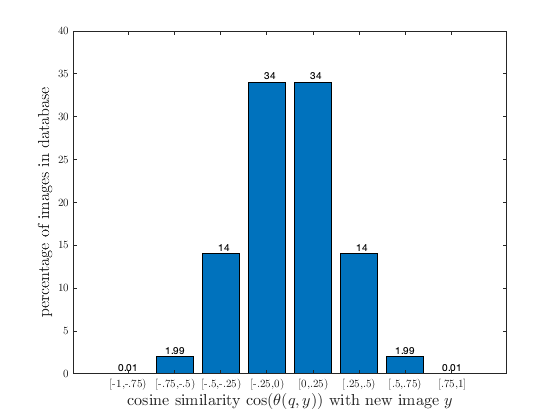
\includegraphics[width=.6\textwidth]{dist.png}
\end{figure} 

Pinterest wants to consider two possible computational targets for your LSH scheme, which will determine the speed of the de-duplication algorithm:
\begin{enumerate}
	\item Ensure that no more than $1$ million candidate near-duplicates are checked on average when a new image is pinned. Here ``checked'' means directly compared against the new image for high cosine similarity.
	\item Ensure that no more than $200,000$ candidates are checked on average when a new image is pinned.
\end{enumerate}

\noindent Based on the data above, describe how to set parameters for your LSH scheme to minimize the space (i.e., number of tables) used, while achieving each of the above goals. Justify your answers, and any assumptions you make.
If you code anything up to help calculate your answer, please attach the code. As in lecture, you can assume that each hash table has $m = O(N)$ slots and this is large enough to ignore lower order terms depending on $1/m$. 





\end{document}